\section{Introduction}

\subsection{Motivation}
\frame{
  \frametitle{Dense SLAM with B-Splines}

  \begin{figure}[]
    \centering
    \begin{subfigure}{.49\linewidth}
      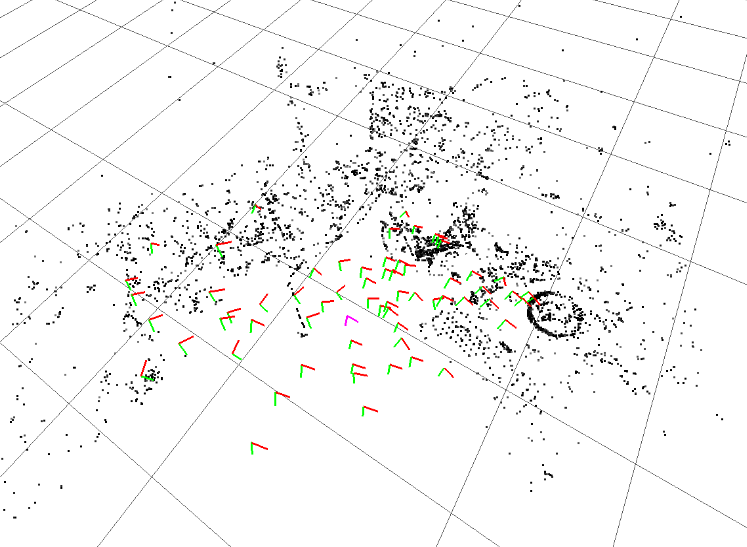
\includegraphics[width=\linewidth]{figures/sparse.png}
        \caption{Sparse SLAM (PTAM, \cite{PTAM})}
    \end{subfigure}
    \begin{subfigure}{.49\linewidth}
      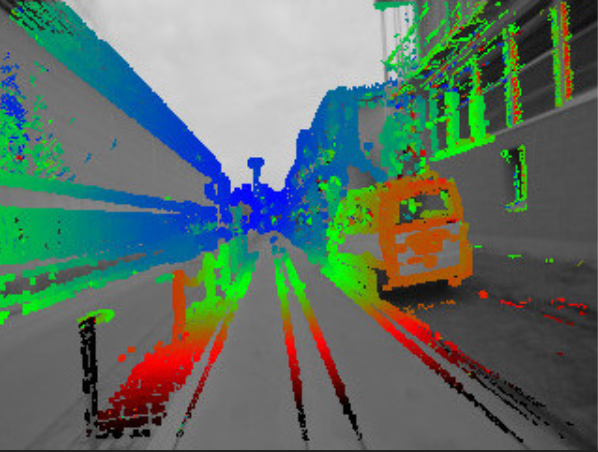
\includegraphics[width=\linewidth]{figures/dense.png}
        \caption{Dense SLAM (LSD-SLAM, \cite{LSD-SLAM})}
    \end{subfigure}
  \end{figure}
}

\subsection{Project Goals}
\frame{
  \frametitle{Stereo Surface Reconstruction And Localization}

  Create framework for surface reconstruction and localization using moving
  stereo camera. 

  \begin{itemize}
    \item \textit{Added functionalities}
    \begin{itemize}
      \item Create spline surface reprensentation from static stereo camera.  
      \item Localize new stereo camera position using obtained map.
    \end{itemize}

  \item \textit{Methodology}
    \begin{itemize}
      \item \textbf{Simulation environment}: \ros with \rviz for pointcloud and
      \opencv for image handling.
    \item \textbf{Optimization}: own implementation of optimization algorithm using \eigen 's sparse matrix solvers.
    \item \textbf{Hardware}: stereo camera data from \rovio sensor,
      \textit{MacBook Pro} with Intel Core 2.7MHz, 4 cores.
    \end{itemize}
\end{itemize}
}
